\section{Introduction}\label{introduction}

This thesis explores the generation of user interfaces (UIs) for application programming interfaces (APIs) that fulfill certain criteria in the context of the World Wide Web. The main goal is to reduce the manual work required in UI development. With this thesis I propose practices and principles to reduce manual work and I implement a proof of concept framework to research the potential of UI generation.

\subsection{Context}\label{context}
In order for information systems to be useful, they either have to interact with other systems or with users. Those systems are increasingly connected together and they exchange data without any human interaction. When it comes to human-computer interaction, UIs are implemented that often consume HTTP APIs which use the JSON data format \citep{jsonformat}. Those UIs are part of mobile, desktop or browser-only applications. End users interact with those client applications through UIs in order to carry out tasks.

\subsection{Problem}\label{problem}
The contemporary way of implementing those UIs involves a lot of manual work. JSON is a very popular data format for infromation systems in web development. While humans can often infer the meaning of a piece of JSON data, it is not trivial for machines to do so. Specific knowledge about the JSON data is needed for a machine to understand the meaning of JSON data. That specific knowledge is only valid for a certain API in a certain context. It is manually, often implicitely, encoded into the applications which contain the UIs. This knowledge is required by a machine to understand the data coming from such an API, it gives the data its \textbf{semantics}. These client applications are strongly coupled to specific APIs and can not be re-used. Instead, new client applications are written each for the end user and for the administrator. New client applications are written for each new project that has its own new data model.

Current approaches fail to exploit the architecture of the World Wide Web and they completely ignore the possibilities offered by \textbf{linked data}.

TODO task based computing

\begin{figure}[!htb]
  \center{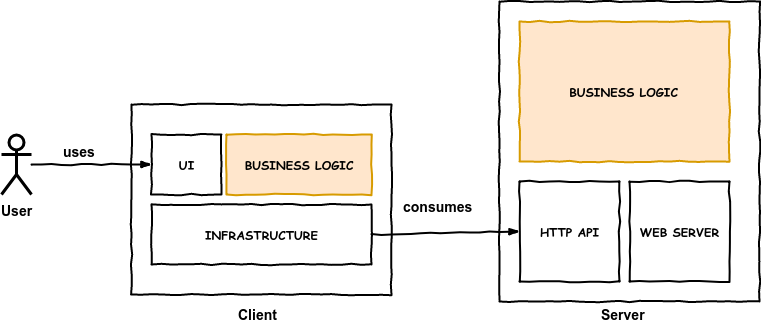
\includegraphics[width=450]
    {images/ui-dev-now.png}}
  \caption{\label{fig:my-label} A part of the business logic is hard coded into the client.}
\end{figure}


\subsection{Strategy}\label{strategy}
The main goal of this thesis is to reduce the amount of manual work by leveraging linked data and the interaction model of task-based computing.
This thesis provides a set of practices, technological building blocks and a proof of concept tool to generate UIs for APIs that conform to a certain specificaction. It build on-top of existing research, work and tools. There is a useful set of building blocks that have not been put together yet in a way, so that it solves the problem of UI generation. The UI framework should work with existing APIs after only slight adjustment. It should provide sane defaults and it should be extensible by developers.

This thesis brings together linked data, existing hyermedia vocabularies and web component-style rendering. The development of the UI framework is done in three iterations, each one solving one artificial UI use-case.

TODO split between rendering (query) and interactions (command)
